\section{Gegnererkennung}
\begin{frame}
\frametitle{\,}
Wurde grösstenteils während der Semesterarbeit erstellt.\\
Ausmessung der Sensoren und Distanzapproximation:
\begin{figure}
	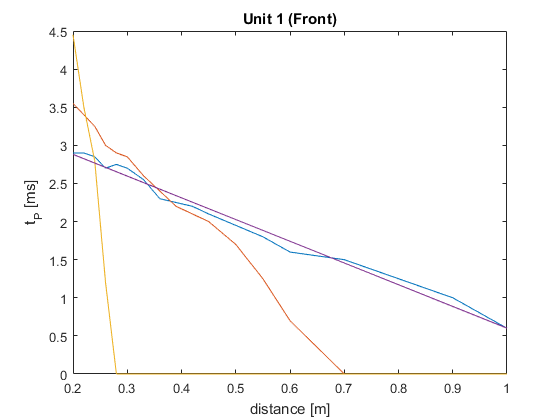
\includegraphics[height = 4 cm]{../images/presentation/OD/FRONT_1.png}
	\hspace{2em}
	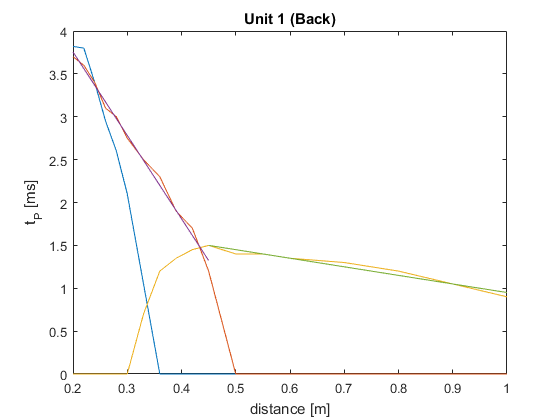
\includegraphics[height = 4 cm]{../images/presentation/OD/BACK_1.png}\\
	\textcolor{yellow}{Near-Sensor}, \textcolor{red}{Middle-Sensor}, \textcolor{cBlue}{Wide-Sensor}
\end{figure}

\end{frame}